\chapter{Landasan Teori}
\label{chap:landasanteori}


Bab ini terdiri atas empat bagian, yaitu Google Authentication, Markdown Syntax, StrapdownJS dan Zurb Foundation. Empat bagian terebut akan membahas mengenai dasar-dasar teori mengenai Google Authentication, Markdown Syntax, StrapdownJS dan Zurb Foundation yang akan digunakan dalam penelitian ini untuk membangun perangkat lunak Sistem Informasi Riwayat Mahasiswa.

\section{Google Authentication \cite{Oauth:2013}}
\label{sec:googleauthentication}

API Google menggunakan protokol OAuth 2.0 untuk otentikasi dan otorisasi. OAuth 2.0 adalah protokol yang relatif sederhana. Untuk memulainya cukup dengan mendapatkan kepercayaan OAuth 2.0 dari Google Developers Console\footnotemark[1]. Maka aplikasi akan meminta suatu token akses dari Google Authorization Server, ekstrak token akses yang merupakan jawaban dari server, dan mengirim token akses ke Google API yang akan diakses.

\footnotetext[1]{https://console.developers.google.com/}
\footnotetext[2]{https://developers.google.com/accounts/docs/OpenIDConnect}

Sub bab berikut memberikan gambaran skenario otorisasi OAuth 2.0 yang merupakan dukung dari Google. Rincian tentang cara menggunakan OAuth 2.0 untuk otentikasi (yaitu sign-in), dapat dilihat pada OpenID Connect\footnotemark[2].

\subsection{Langkah Dasar}
Semua aplikasi akan mengikuti pola dasar ketika menggakses Google API menggunakan Oauth 2.0. Terdapat empat langkah yang harus diikuti :

\begin{enumerate}
\item
Mendapatkan kepercayaan OAuth 2.0 dari Google Developers Console\\
Berkunjung ke Google Developers Console untuk mendapatkan kepercayaan OAuth 2.0 seperti klien id dan kerahasiaan klien yang keduanya dikenal oleh Google dan aplikasi yang dibuat. Set nilai-nilai yang bervariasi sesuai dengan jenis aplikasi apa yang sedang dibuat. Misalnya, sebuah aplikasi javascript tidak memerlukan sebuah rahasia, tapi apakah aplikasi web server memerlukannya.
\item
Memperoleh token akses dari Google Authorization Server\\
Sebelum aplikasi dapat mengakses data privat dengan menggunakan Google API, terlebih dahulu diperlukan token akses untuk mengakses API tersebut. Satu token akses dapat memberikan berbagai tingkat akses ke beberapa API. Izin token akses merupakan parameter untuk variabel ruang lingkup yang mengontrol sumber daya dan operasi. Selama ada permintaan untuk token akses, maka aplikasi akan mengirimkan satu atau lebih nilai pada parameter ruang lingkup.

Ada beberapa cara dan variasi untuk melakukan permintaan tersebut berdasarkan aplikasi yang dibangun. Contohnya aplikasi JavaScript mungkin meminta token akses menggunakan mesin pencari yang mengarah kembali ke Google, namun aplikasi yang dibangun diinstal pada perangkat tidak memiliki fitur mesin pencari maka akan menggunakan {\it web service}. Beberapa permintaan memerlukan tahap otentikasi dimana pengguna diharuskan login menggunakan akun Google mereka. Setelah login pengguna akan ditanya apakah pengguna akan memberi izin untuk aplikasi yang telah melakukan permintaan tersebut. Proses ini disebut izin dari pihak pengguna. Jika pengguna memberi izin, maka Google Authorization Server akan mengirimkan aplikasi tersebut sebuah token akses. Jika pengguna tidak memberi izin, maka server akan menunjukan respon yang menyatakan eror.
\item
Kirim token akses ke API\\
Setelah aplikasi mendapat token akses, lalu aplikasi akan mengirimkan token akses ke Google API melalui otorisasi yang terletak pada header HTTP. Sangat mungkin untuk mengirimkan token sebagai parameter permintaan URI dalam tipe data {\it string}, namun langkah ini tidak direkomendasikan karena parameter URI akan berakhir pada file log yang tidak aman. Juga merupakan hal yang baik karena menghindari menciptakan nama parameter URI yang tidak perlu.
Token akses hanya berlaku untuk set operasi dan sumber daya yang dijelaskan pada lingkup permintaan token. Sebagai contoh, jika token akses dikeluarkan untuk Google+ API, hal tersebut tidak memberikan akses untuk Google Contact API. Namun token akses untuk Google+ API dapat dikirim beberapa kali untuk operasi yang serupa.
\item
Memperbaharui token akses jika diperlukan\\
Token akses memiliki daya tahan yang terbatas. Jika aplikasi yang dibangun membutuhkan akses ke Google API melebihi masa aktif token akses, maka dapat memperbaharui token akses tersebut. Hal ini memungkinkan untuk memdapatkan token akses yang baru.
\end{enumerate}

\subsection{Skenario Aplikasi Web Server}
Google OAuth 2.0 mendukung aplikasi web server yang menggunakan bahasa dan kerangka kerja seperti PHP, Java, Python, Ruby, dan ASP.NET.

Urutan otorisasi dimulai ketika aplikasi mengarahkan mesin pencari ke URL Google; URL tersebut termasuk parameter permintaan yang menunjukkan jenis akses yang diminta. Google menangani otentikasi pengguna, pemilihan sesi, dan izin dari pihak pengguna. Hasilnya adalah sebuah kode otorisasi, dimana aplikasi dapat bertukar untuk token akses dan memperbaharui token akses.

Aplikasi harus menyimpan pembaharuan token akses untuk penggunaan kedepannya dan menggunakan token akses untuk mengakses Google API. Setelah masa token akses berakhir, maka aplikasi akan memperbaharui token akses untuk mendapatkan yang baru. Untuk gambaran skenario dapat dilihat pada Gambar \ref{fig:skenarioaplikasiwebserver}.

\begin{figure}[H]
\centering
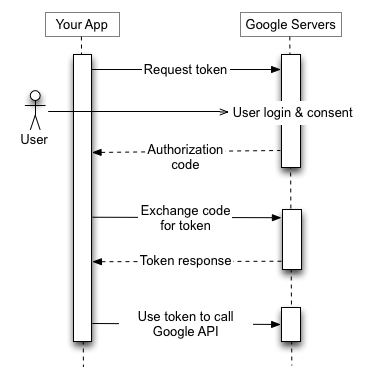
\includegraphics[scale=1]{Gambar/skenario1.png}
\caption[Gambar Skenario Aplikasi Web Server]{Skenario Aplikasi Web Server} 
\label{fig:skenarioaplikasiwebserver}
\end{figure}

\subsection{Skenario Aplikasi yang Terinstal}
Google OAuth 2.0 mendukung aplikasi yang diinstal pada perangkat seperti komputer, perangkat mobile, dan tablet. Ketika membuat klien id melalui Google Developers Console, menentukan aplikasi yang terinstal kemudian pilih Android, Chrome, iOS, atau "{\it Other}" sebagai jenis aplikasi.

Hasil proses klien id dan kerahasiaan klien dalam beberapa kasus dimasukkan dalam kode sumber aplikasi. (Dalam konteks ini, kerahasiaan klien jelas tidak diperlakukan sebagai rahasia.)

Urutan otorisasi dimulai ketika aplikasi mengarahkan mesin pencari ke URL Google; URL termasuk parameter permintaan yang menunjukkan jenis akses yang diminta. Google menangani otentikasi pengguna, pemilihan sesi, dan izin pengguna. Hasilnya adalah sebuah kode otorisasi yang dapat bertukar untuk token akses dan memperbaharui token.

Aplikasi harus menyimpan token yang diperbaharui untuk penggunaan masa depan dan menggunakan token akses untuk mengakses API Google. Setelah masa token akses berakhir, maka aplikasi akan memperbaharui token untuk mendapatkan yang baru. Untuk gambar skenario dapat dilihat pada Gambar \ref{fig:skenarioaplikasiyangterinstal}.

\begin{figure}[H]
\centering
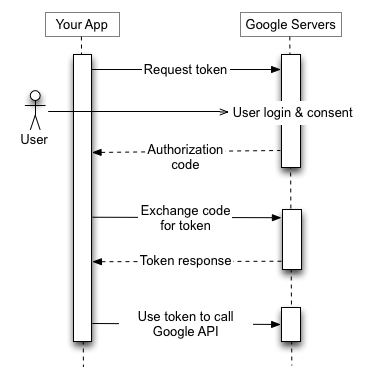
\includegraphics[scale=1]{Gambar/skenario1.png}
\caption[Gambar Skenario Aplikasi yang Terinstal]{Skenario Aplikasi yang Terinstal} 
\label{fig:skenarioaplikasiyangterinstal}
\end{figure}

\subsection{Skenario Aplikasi Sisi Klien (JavaScript)}
Google OAuth 2.0 mendukung aplikasi JavaScript yang berjalan di mesin pencari. Urutan otorisasi dimulai ketika aplikasi mengarahkan mesin pencari ke URL Google; URL termasuk parameter permintaan yang menunjukkan jenis akses yang diminta. Google menangani otentikasi pengguna, pemilihan sesi, dan izin pengguna. Hasilnya adalah token akses dimana klien harus memvalidasi sebelum memasukkannya ke dalam permintaan Google API. Ketika masa token berakhir, aplikasi mengulangi proses. Untuk gambar skenario dapat dilihat pada Gambar \ref{fig:skenarioaplikasisisiklien}.

\begin{figure}[H]
\centering
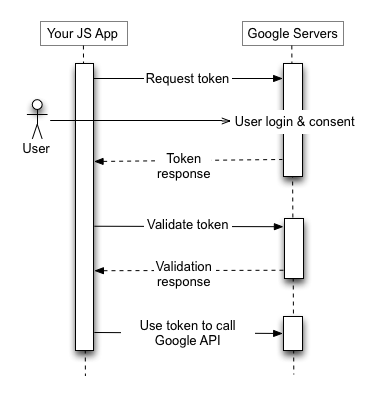
\includegraphics[scale=1]{Gambar/skenario2.png}
\caption[Gambar Skenario Aplikasi Sisi Klien (JavaScript)]{Skenario Aplikasi Sisi Klien (JavaScript)}
\label{fig:skenarioaplikasisisiklien}
\end{figure}

\subsection{Skenario Aplikasi Pada Perangkat Dengan Masukan Yang Terbatas}
Google OAuth 2.0 mendukung aplikasi yang berjalan pada perangkat dengan masukan yang terbatas seperti konsol game, kamera video, dan printer. Urutan otorisasi dimulai dengan aplikasi membuat permintaan layanan web ke URL Google untuk kode otorisasi. Tanggapan berisi beberapa parameter, termasuk URL dan kode bahwa aplikasi menunjukkan kepada pengguna. Pengguna memperoleh URL dan kode dari perangkat, kemudian beralih ke perangkat terpisah atau komputer dengan kemampuan masukan yang lebih. Pengguna membuka mesin pencari, menavigasi ke URL tertentu, melakukan log in, dan memasukan kode.

Sementara itu, aplikasi jajak pendapat dari URL Google pada interval tertentu. Setelah pengguna menyetujui akses, respon dari server Google berisi token akses dan memperbaharui token. Aplikasi harus menyimpan token yang baru untuk penggunaan masa depan dan menggunakan token akses untuk mengakses Google API. Setelah masa token akses berakhir, maka aplikasi akan memperbaharui token untuk mendapatkan yang baru. Untuk gambar skenario dapat dilihat pada Gambar \ref{fig:skenarioaplikasimasukanterbatas}.

\begin{figure}[H]
\centering
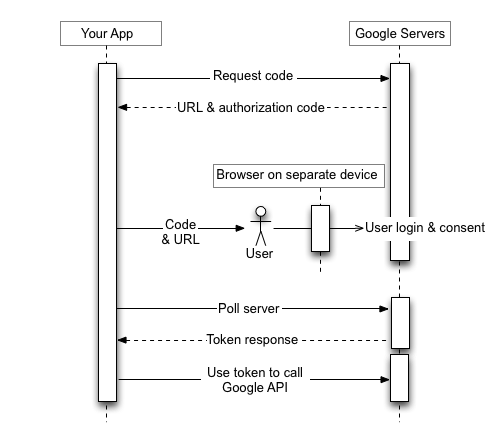
\includegraphics[scale=1]{Gambar/skenario3.png}
\caption[Gambar Skenario Aplikasi Pada Perangkat Dengan Masukan Yang Terbatas]{Skenario Aplikasi Pada Perangkat Dengan Masukan Yang Terbatas}
\label{fig:skenarioaplikasimasukanterbatas}
\end{figure}

\subsection{Skenario Layanan Akun}
Google API seperti Prediction API dan Google Cloud Storage dapat bertindak atas nama aplikasi yang dibuat tanpa mengakses informasi pengguna. Dalam situasi ini aplikasi perlu membuktikan identitasnya sendiri ke API, tapi tidak diperlukan izin dari pihak pengguna. Demikian pula, dalam skenario perusahaan, aplikasi dapat meminta akses didelegasikan ke beberapa sumber daya.

Untuk jenis interaksi antara server memerlukan layanan akun, dimana akun tersebut terdapat pada aplikasi yang dibuat, bukan individu ke pengguna akhir. Aplikasi memanggil Google API atas nama layanan akun, dan izin dari pihak pengguna tidak diperlukan. (Dalam skenario tanpa layanan akun, aplikasi memanggil Google API atas nama pengguna akhir, dan izin dari pihak pengguna kadang-kadang diperlukan.)

Catatan: skenario layanan akun ini membutuhkan aplikasi untuk membuat dan tanda kriptografi JSON Web Token (JWTs). Sangat disarankan untuk menggunakan perpustakaan untuk melakukan tugas-tugas ini. Jika menulis kode ini tanpa menggunakan perpustakaan secara abstrak tanda penciptaan dan penandatanganan, mungkin membuat kesalahan yang akan memiliki dampak yang parah pada keamanan aplikasi yang dibangun.

Kredensial ayanan akun , yang diperoleh dari Google Developers Console, termasuk alamat email yang dihasilkan yang unik, klien id, dan setidaknya satu pasang kunci publik / privat. Menggunakan klien id dan satu kunci privat untuk membuat JWT ditandatangani dan membangun permintaan token akses dalam format yang sesuai. Aplikasi kemudian mengirimkan permintaan token ke Google OAuth 2.0 Authorization Server, yang mengembalikan token akses. Aplikasi menggunakan token untuk mengakses API Google. Ketika masa token berakhir, aplikasi mengulangi proses. Untuk gambar skenario dapat dilihat pada Gambar \ref{fig:skenariolayananakun}.

\begin{figure}[H]
\centering
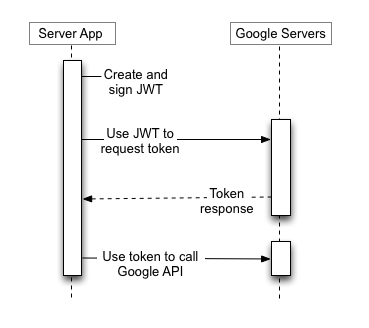
\includegraphics[scale=1]{Gambar/skenario4.png}
\caption[Gambar Skenario Layanan Akun]{Skenario Layanan Akun}
\label{fig:skenariolayananakun}
\end{figure}

\subsection{Masa Habis Berlaku Token}
Kode token harus ditulis untuk mengantisipasi kemungkinan bahwa token yang diberikan mungkin tidak lagi bekerja suatu saat. Token mungkin berhenti bekerja untuk beberapa alasan di bawah ini:

\begin{itemize}
\item
Pengguna telah mencabut akses.
\item
Token tidak digunakan selama enam bulan.
\item
Akun pengguna telah melampaui jumlah tertentu permintaan token.
\end{itemize}

Saat ini batas untuk setiap akun Google adalah 25 token. Jika pengguna akun telah memiliki 25 token, permintaan otentikasi untuk token ke-26 akan berhasil tapi token yang paling tua atau token ke-1 akan dibuat tidak berlaku tanpa sepengetahuan pengguna.
Jika perlu untuk mengotorisasi beberapa program, mesin, atau perangkat, salah satu solusi adalah untuk membatasi jumlah klien dimana harus mengotorisasi per pengguna akun antara 15 atau 20. Jika Anda adalah admin Google Apps, Anda dapat membuat admin tambahan untuk mengizinkan beberapa klien.

\section{Markdown \cite{Markdown:2015}}
\label{sec:markdown}

Markdown memungkinkan untuk menulis agar mudah dibaca dan mudah ditulis dalam format teks biasa. Kemudian diubah menjadi HTML yang valid seperti contoh dapat dilihat pada GitHub. 

\subsection{Dasar Penulisan}
Terdapat empat hal yang ada didalam dasar penulisan, empat hal tersebut dapat dilihat dibawah ini. 

\begin{enumerate}
\item Paragraf\\
Paragraf dalam Markdown merupakan satu atau lebih baris teks berturut-turut yang diikuti oleh satu atau lebih baris kosong.
\begin{lstlisting}
On July 2, an alien mothership entered Earth's orbit and deployed several dozen saucer-shaped "destroyer" spacecraft, each 15 miles (24 km) wide.

On July 3, the Black Knights, a squadron of Marine Corps F/A-18 Hornets, participated in an assault on a destroyer near the city of Los Angeles.
\end{lstlisting}
\item Judul Sub Bab\\
Titel dapat dibuat dengan menambahkan satu atau lebih simbol \# sebelum teks titel. Jumlah \# yang digunakan akan menentukan ukuran titel.
\begin{lstlisting}
# The largest heading (an <h1> tag)
## The second largest heading (an <h2> tag)
### The third largest heading (an <h3> tag)
#### The 4th largest heading (an <h4> tag)
##### The 5th largest heading (an <h5> tag)
###### The 6th largest heading (an <h6> tag)
\end{lstlisting}
\item {\it Blockquotes}\\
{\it Blockquotes} dapat ditunjukkan dengan simbol >.
\begin{lstlisting}
In the words of Abraham Lincoln:

> Pardon my french
\end{lstlisting}
\item Gaya teks\\
Gaya teks yang dapat dibuat adalah teks tebal atau miring.
\begin{lstlisting}
*This text will be italic*
**This text will be bold**
\end{lstlisting}
\end{enumerate}

\subsection{Daftar}
Terdapat tiga macam daftar yang dapat dibuat. Tiga macam daftar tersebut dapat dilihat dibawah ini.

\begin{enumerate}
\item Daftar tidak berurutan\\
Untuk membuat daftar tidak berurutan dapat menggunakan simbol bintang * maupun simbol - sebelum daftar item.
\begin{lstlisting}
* Item
* Item
* Item

- Item
- Item
- Item
\end{lstlisting}
\item Daftar berurutan\\
Untuk membuat daftar berurutan dapat menggunakan nomor sebelum daftar item.
\begin{lstlisting}
1. Item 1
2. Item 2
3. Item 3
\end{lstlisting}
\item Daftar bersarang\\
Daftar bersarang dapat dibuat dengan identifikasi daftar item dengan dua spasi.
\begin{lstlisting}
1. Item 1
  1. A corollary to the above item.
  2. Yet another point to consider.
2. Item 2
  * A corollary that does not need to be ordered.
    * This is indented four spaces, because it's two spaces further than the item above.
    * You might want to consider making a new list.
3. Item 3
\end{lstlisting}
\end{enumerate}

\subsection{Format Kode}

\begin{enumerate}
\item Format Sebaris\\
Menggunakan tanda kutip mundur tunggal (`) untuk memformat teks dalam format monospace khusus. Segala sesuatu dalam tanda kutip mundur muncul sebagai-adalah, tanpa format khusus lainnya.
\begin{lstlisting}
Here's an idea: why don't we take `SuperiorProject` and turn it into `**Reasonable**Project`.
\end{lstlisting}
\item Format Beberapa Baris\\
Anda dapat menggunakan tanda kutip mundur tiga (```) untuk memformat teks sebagai blok sendiri yang berbeda.
\begin{lstlisting}
Check out this neat program I wrote:

```
x = 0
x = 2 + 2
what is x
```
\end{lstlisting}
\end{enumerate}

\subsection{Link}
Anda dapat membuat link inline dengan membungkus link teks dalam tanda kurung ( [ ] ), dan kemudian membungkus link dalam tanda kurung ( ( ) ).
Misalnya, untuk membuat hyperlink ke www.github.com, dengan teks link yang mengatakan, Visit GitHub !, Anda akan menulis ini dalam Markdown: [Kunjungi GitHub!] (www.github.com).

\section{StrapdownJS \cite{Strapdownjs:2014}}
\label{sec:stapdownjs}

Strapdown.js membuat lebih sederhana untuk membuat dokumen Markdown yang elegan. Tidak diperlukan kompilasi dari sisi server. Gunakan strapdown.js untuk mendokumentasikan proyek dengan cepat, membuat tutorial, membuat halaman utama sebuah website. Contoh website yang menggunakan strapdown.js adalah http://strapdownjs.com/.

Cukup salin template HTML dibawah ini dan taruh pada file server statis :
\begin{lstlisting}
<!DOCTYPE html>
<html>
<title>Hello Strapdown</title>

<xmp theme="united" style="display:none;">
# Markdown text goes in here

## Chapter 1

Lorem ipsum dolor sit amet, consectetur adipisicing elit, sed do eiusmod tempor incididunt ut labore
et dolore magna aliqua. 

## Chapter 2

Ut enim ad minim veniam, quis nostrud exercitation ullamco laboris nisi ut
aliquip ex ea commodo consequat. Duis aute irure dolor in reprehenderit in voluptate velit esse
cillum dolore eu fugiat nulla pariatur. Excepteur sint occaecat cupidatat non proident, sunt in
culpa qui officia deserunt mollit anim id est laborum.
</xmp>

<script src="http://strapdownjs.com/v/0.2/strapdown.js"></script>
</html>
\end{lstlisting}

Strapdonw.js juga memiliki beberapa fitur :
\begin{enumerate}
\item Ramah dengan mesin pencari
\item Kompatibel dengan berbagai browser (Sudah diuji dengan ponsel menggunakan Safari, IE 8/9, Firefox, Chrome)
\item Github menggunakan Markdown (Tabel, Syntax, Headline)
\item Dapat menggunakan tema
\end{enumerate}

\section{Zurb Foundation \cite{Zurb:2015}}
\label{sec:zurbfoundation}

Zurb Foundation merupakan alat bantu dalam membuat aplikasi baru maupun membuat website yang responsif. Jutaan desainer dan teknisi menggunakan Foundation sebagai bagian dari alur kerja mereka. Zurb Foundation adalah {\it framework} pertama yang memperkenalkan konsep responsif, semantik, mobile dan parsial. Zurb Foundation juga kompatibel dengan kebanyakan mesin pencari dan perangkat. Maka dari itu Zurb Foundation merupakan pilihan profesional bagi para desainer dan teknisi.

\subsection{Kompatibilitas}
Zurb Foundation dirancang dan diuji pada berbagai browser dan perangkat. Daftar pengujian pada berbagai browser dan perangkat dapat dilihat pada Tabel \ref{tab:kompatibilitas}.

\newcommand{\cmark}{\ding{51}}%
\newcommand{\xmark}{\ding{55}}%
\begin{center}
\begin{table}
\caption[Tabel 2-1 Daftar Pengujian Zurb Foundation]{Daftar Pengujian Zurb Foundation\footnotemark[1]}\\
\label{tab:kompatibilitas}
\begin{center}
\begin{tabular}{|l|l|1|l|}
\hline
Browser/OS & The Grid & Layout/UI & JS\\
\hline
Chrome & \cmark & \cmark & \cmark\\
\hline
Firefox & \cmark & \cmark & \cmark\\
\hline
Safari & \cmark & \cmark & \cmark\\
\hline
IE10 & \cmark & \cmark & \cmark\\
\hline
IE11 & \cmark & \cmark & \cmark\\
\hline
IE9 & \cmark & \cmark & \cmark\\
\hline
IE8 & \xmark & \xmark & \xmark\\
\hline
IE7 & \xmark & \xmark & \xmark\\
\hline
iOS (iPhone) & \cmark & \cmark & \cmark\\
\hline
iOS (iPad) & \cmark & \cmark & \cmark\\
\hline
Android 2, 4 (Phone) & \cmark & \cmark & \cmark\\
\hline
Android 2, 4 (Tablet) & \cmark & \cmark & \cmark\\
\hline
Windows Phone 7+ & \cmark & \cmark & \cmark\\
\hline
Surface & \cmark & \cmark & \cmark\\
\hline
\end{tabular}
\end{center}
\end{table}
\end{center}

\footnotetext[1]{http://foundation.zurb.com/docs/compatibility.html}
\footnotetext[2]{http://foundation.zurb.com/docs/components/kitchen_sink.html#js}

\subsection{Apa Saja yang Hadir Dengan Foundation?}
Foundation memiliki banyak komponen dan struktur untuk membantu membangun sebuah situs responsif. Semua komponen Foundation dapat dilihat pada satu halaman yang disebut Kitchen Sink\footnotemark[2] atau melihat beberapa gambar dibawah ini :

\begin{enumerate}
\item The Grid\\
Grid bekerja pada hampir semua perangkat dan memiliki dukungan untuk menjadi satu kesatuan, sumber pemesanan, offset dan perangkat presentasi. Hal tersebuat sedikit terlalu mudah, dalam waktu singkat, dapat menciptakan tata letak yang kompleks seperti ini. Untuk contoh grid dapat dilihat pada Gambar \ref{fig:grid}.

\begin{figure}[H]
\centering
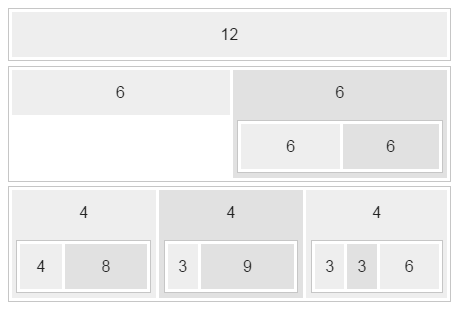
\includegraphics[scale=1]{Gambar/grid.png}
\caption[Gambar Contoh Grid]{Contoh Grid}
\label{fig:grid}
\end{figure}

\item Tombol\\
Mengklik tombol dengan material yang bagus merupakan hal yang mengagumkan. Mengklik tombol juga menghubungkan pengguna dengan berbagai aksi. Ada beberapa gaya tombol yamg ringan untuk ukuran, presentasi, dan warna untuk menyesuaikan tombol Anda sendiri semudah menambahkan kelas. Untuk contoh macam-macam tombol dapat dilihat pada Gambar \ref{fig:button}.

\begin{figure}[H]
\centering
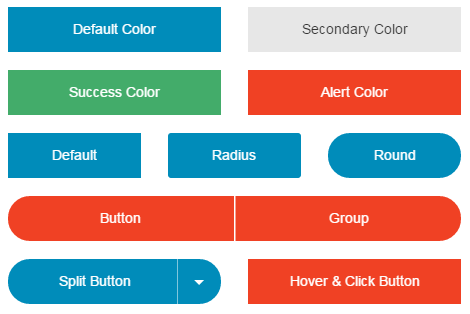
\includegraphics[scale=1]{Gambar/button.png}
\caption[Gambar Contoh Tombol]{Contoh Tombol}
\label{fig:button}
\end{figure}

\item Navigasi\\
Orang yang mengakses harus bisa berkeliling melihat menu-menu yang ada. Gaya navigasi pada Foundation meliputi : bar bagian atas yang kuat dengan menu dropdown; tombol; bar pencari; ikon bar yang keren; implementasi kanvas yang lepas dari keluhan; dan sekelompok navigasi lainnya. Untuk contoh macam-macam navigasi dapat dilihat pada Gambar \ref{fig:navi}.

\begin{figure}[H]
\centering
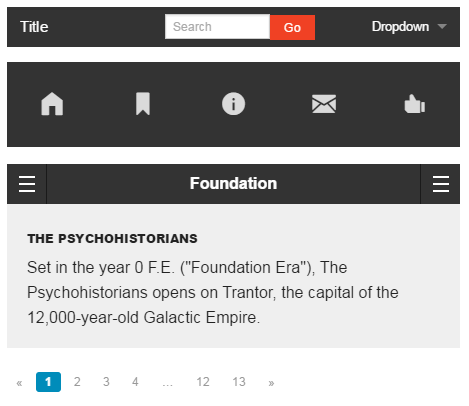
\includegraphics[scale=1]{Gambar/navigation.png}
\caption[Gambar Contoh Navigasi]{Contoh Navigasi}
\label{fig:navi}
\end{figure}

\item Plugins\\
Sudah meliputi banyak plugin javascript yang ditulis untuk modal dasar pop-up; menambat formulir validasi yang diperlukan; membuat tab konten; tanda peringatan; dan masih banyak lagi. Untuk contoh macam-macam plugin dapat dilihat pada Gambar \ref{fig:plugin}.

\begin{figure}[H]
\centering
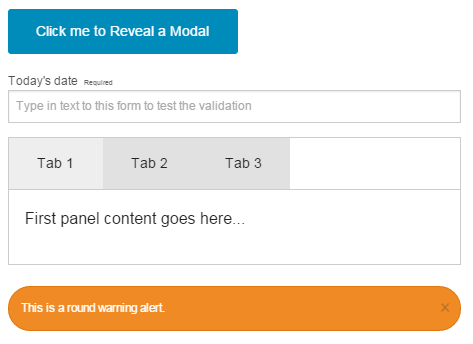
\includegraphics[scale=1]{Gambar/plugin.png}
\caption[Gambar Contoh Plugins]{Contoh Plugins}
\label{fig:plugin}
\end{figure}

\end{enumerate}